\section{Discussion}

\subsection{Particle Swarm Optimisation}

\subsubsection{Convergence analysis}

Across all eight cases, the convergence curves exhibit the characteristic two‑phase behaviour commonly associated with Particle Swarm Optimisation: an initial rapid descent, driven by broad exploration, followed by a slower refinement period once the swarm approaches a promising region of the search space. Despite this shared structure, the rate and extent of convergence vary strongly from one case to another, indicating that each optimisation scenario presents a different level of landscape complexity. Cases 1, 3, 4, and 5 follow relatively long convergence trajectories, with improvements extending over several hundred iterations. Their curves suggest that the cost function contains wider or more intricate basins of attraction, requiring the swarm to progressively refine its position before reaching a stable minimum. In contrast, cases 2, 6, and 8 converge extremely rapidly, stabilising after only a few tens of iterations. This behaviour points to smoother or more accessible optima, where the swarm encounters a well‑defined descent direction early in the search. Case 7 sits between these two trends: it displays a strong initial drop comparable to the fastest‑converging cases, but continues to make gradual improvements up to around 200 iterations, indicating the presence of secondary features in the landscape that delay complete stabilisation. Overall, the variability in convergence rates reflects the heterogeneous nature of the underlying test cases. Rapidly converging cases seem to correspond to simpler or more convex search regions, while slowly converging ones point to more irregular or high‑dimensional surfaces where additional exploration is required. This diversity highlights the importance of assessing convergence behaviour individually rather than assuming uniform optimisation difficulty across cases.

\subsubsection{Profile analysis}

Taken together, the eight optimised profiles illustrate how the cooling‑tower geometry adapts to a wide spectrum of volumetric and boundary conditions. Despite all cases sharing the fundamental hyperbolic identity characteristic of natural‑draft cooling towers, the optimisation outcomes reveal four distinct geometric regimes, each driven by different balances between required height, waist radius, and curvature distribution. The tall and narrow‑waist towers (cases 3 and 6) demonstrate how the optimisation stretches the structure vertically when the available radius is constrained, producing pronounced upper flares to compensate for slender mid‑height sections. The medium‑height towers (cases 4 and 7) represent a more classical hyperbolic shape, where the curvature above and below the waist remains symmetric and structurally coherent. In contrast, cases 1 and 5 converge to almost identical mid‑height profiles, showing that certain target volumes admit a single dominant optimal geometry with limited room for variation. Finally, the most compact and wide‑waist shapes (cases 2 and 8) highlight scenarios where the optimisation requires minimal reshaping, as the volume can be satisfied with little deviation from a cylindrical‑like baseline. Across all regimes, the optimisation systematically redistributes curvature to satisfy the prescribed volume while maintaining smooth, physically meaningful tower contours. This diversity of outcomes reinforces the importance of analysing cooling‑tower profiles not only on the basis of their final area or error metrics but also in terms of their geometric structure, which provides valuable insight into the underlying constraints governing each optimisation scenario.

\subsubsection{Best result}

The choice of the best cooling-tower is based on the following criteria:
\begin{itemize}
    \item \textbf{Volume fidelity:}
    The target volume must be matched as closely as possible. Zero error is preferred; near‑zero is acceptable only if justified by other gains.

    \item \textbf{Convergence behaviour:}
    Fast, monotonic convergence to a stable plateau is required. Late oscillations or very long “creep” phases are penalised as they indicate sensitivity to stochastic effects or a poorly conditioned search landscape.

    \item \textbf{Area:}
    A smaller external envelope generally correlates with lower material use, reduced mass, and potentially lower cost. While structural verification is outside the present scope, area provides a consistent comparative surrogate at this stage.

    \item \textbf{Geometric plausibility of the cooling-tower profile:}
    The optimised profile should be smooth, physically meaningful, and free of abrupt kinks: a coherent hyperbolic silhouette, a reasonable waist, and balanced curvature above and below mid‑height.
\end{itemize}

\begin{figure}[H]
    \centering
    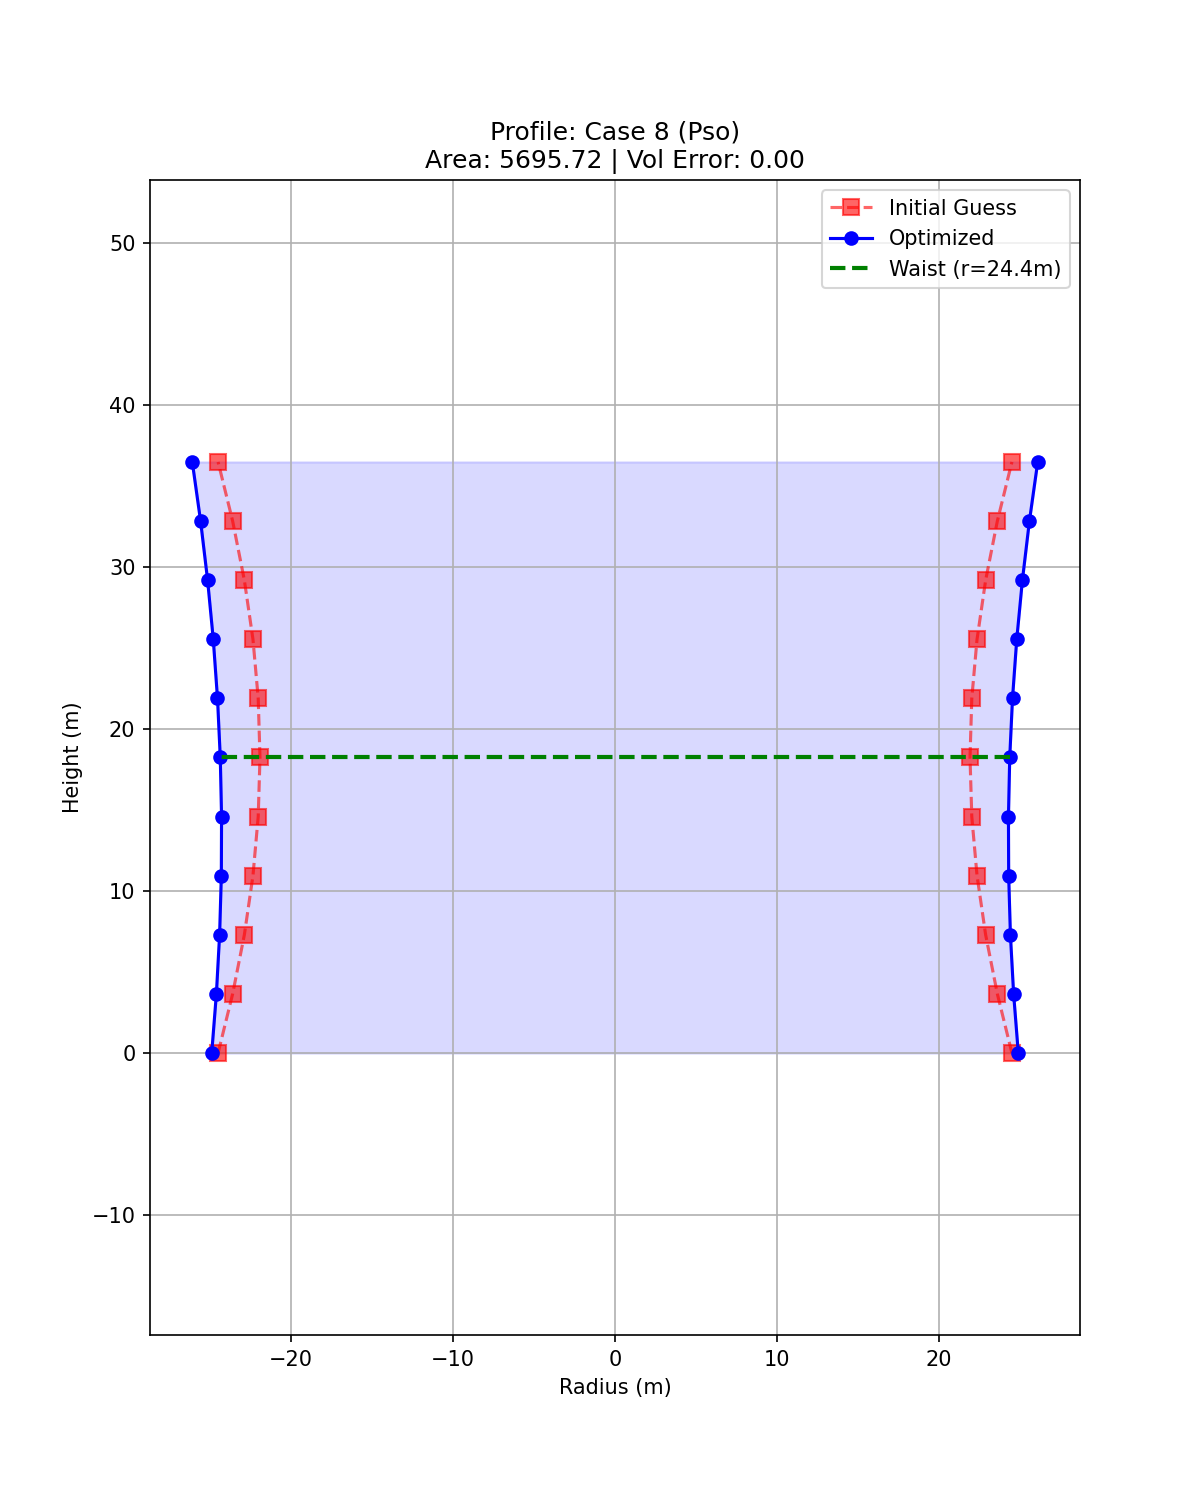
\includegraphics[width=0.50\textwidth]{../Images/PSO/Case8_Pso_profile.png}
    \caption{Best cooling tower with PSO algorithm}
\end{figure}

Based on these criteria, case 8 emerges as the most appropriate cooling‑tower configuration. First, in terms of volume fidelity, case 8 achieves a zero volume error, indicating a perfect match with the prescribed target without requiring compensatory geometric distortions. This level of accuracy is only shared with a small subset of cases, yet case 8 distinguishes itself among them through superior performance on several other dimensions.
Regarding convergence behaviour, case 8 presents one of the cleanest and most rapid convergence histories. The cost function drops sharply within the first iterations and stabilises immediately, showing no signs of late oscillations or prolonged refinement phases. This stable behaviour provides confidence in the robustness of the obtained optimum and reduces the likelihood that the solution is sensitive to stochastic fluctuations. By contrast, some alternative cases with good volume fidelity exhibit longer convergence trajectories or more gradual plateauing, which weakens their comparative reliability.
The area measure also strongly supports the selection of case 8. It yields the smallest external envelope across all eight cases, significantly lower than those of the other zero‑error candidates. As area is used here as a proxy for material and fabrication efficiency, a reduced surface envelope implies a more economical and structurally lightweight design. This advantage is particularly striking when compared with cases 1 and 5, which, despite their excellent volume match, present substantially larger envelopes.
Finally, the geometric plausibility of the resulting cooling‑tower profile reinforces this choice. The optimised shape of  case 8 is smooth, coherent, and free of abrupt curvature transitions, exhibiting a compact silhouette with a consistent radial gradient and a physically realistic waist. Among all the profiles, it is one of the most regular and least distorted, requiring only modest adjustments from the initial guess while still achieving perfect volume compliance.
Taken together, these observations show that case 8 offers the best balance of accuracy, stability, efficiency, and physical credibility. It therefore represents the most defensible choice for the optimal cooling‑tower configuration within the scope of this study.

\subsection{SA}

\subsection{BFGS}

\subsection{Global discussion}
